\documentclass[12pt]{beamer}
%
% Choose how your presentation looks.
%
% For more themes, color themes and font themes, see:
% http://deic.uab.es/~iblanes/beamer_gallery/index_by_theme.html
%
\mode<presentation>
{
  \usetheme{Berkeley}      % or try Darmstadt, Madrid, Warsaw, ...
  \usecolortheme{default} % or try albatross, beaver, crane, ...
  \usefonttheme{structurebold}  % or try serif, structurebold, ...
  \setbeamertemplate{navigation symbols}{}
  \setbeamertemplate{caption}[numbered]
} 

\usepackage[english]{babel}
\usepackage[utf8]{inputenc}
% \usepackage{graphicx}
\usepackage{verbatim}
\usepackage{multicol}
\usepackage{enumitem}

\title{Autocell}
%\subtitle{A game to sell auto parts}
\author{Bryant Benzant-Ortiz}
\date{\today}

\begin{document}

\begin{frame}
  \titlepage
\end{frame}

\begin{frame}{New Approach to Marketing}
	You see marketing in games such as mobile games on your phone
	\begin{itemize}
		\item Advergames -- games where you play on the phone as an advertisement to get consumers into downloading the game after a demo
	\end{itemize}
\end{frame}

\begin{frame}{New Game}
	What is Autocell?

	Autocell is a new game idea where the advertisements are in the game.

	The theme of the selling product is Car Parts.

	The kind of advertisements that this game will use is some brand names in car parts. There are car models that are actual models from real world brands. 

	The purpose of this game is for players, as consumers, to create a vehicle and experiment with car parts on which ones are better for a sedan.
\end{frame}
%\begin{frame}{Gameplay}
%	
%\end{frame}
\begin{frame}{}
	\centering\textsc{\textbf{Demo}}
\end{frame}
\begin{frame}{Software Used}
	\begin{multicols}{2}
	\begin{itemize}[nosep,noitemsep]
		\item Unity
		\item C\#
		\item Blender
	\end{itemize}
	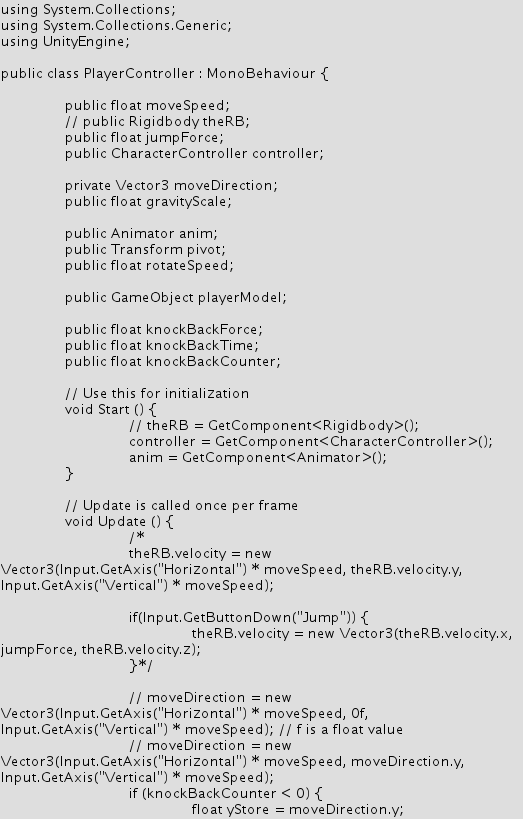
\includegraphics[height=2.75in]{Code}
	\end{multicols}
\end{frame}
\begin{frame}{Summary}
	Things to do for the future:
	\begin{itemize}
		\item Make some levels
		\item Generate a city for the player to explore
		\item Make a coverflow shop with the brands shown in each cell
	\end{itemize}
\end{frame}
\begin{frame}{}
	\centering\textsc{\textbf{Comments}}
\end{frame}

\end{document}
